% Asset ID: FAS1ConicSections1TikZ-003
% Source: FP1-Chp2-ConicSections1.pdf chord example
% Purpose: Show the vertical chord produced when x = k cuts y^2 = 4ax.
\documentclass[tikz,border=6pt]{standalone}
\usepackage{amsmath}
\usepackage{xcolor}
\usetikzlibrary{arrows.meta,calc,decorations.pathreplacing,backgrounds}
\definecolor{canvas}{HTML}{FAF9F6}
\definecolor{ivory}{HTML}{FFFFF0}
\definecolor{linegray}{HTML}{E5E5EA}
\definecolor{gold}{HTML}{C5A059}
\definecolor{ink}{HTML}{2C2C2E}
\definecolor{rose}{HTML}{FBEFEF}
\definecolor{teal}{HTML}{6B9FA3}
\definecolor{purple}{HTML}{8F6C9F}
\begin{document}
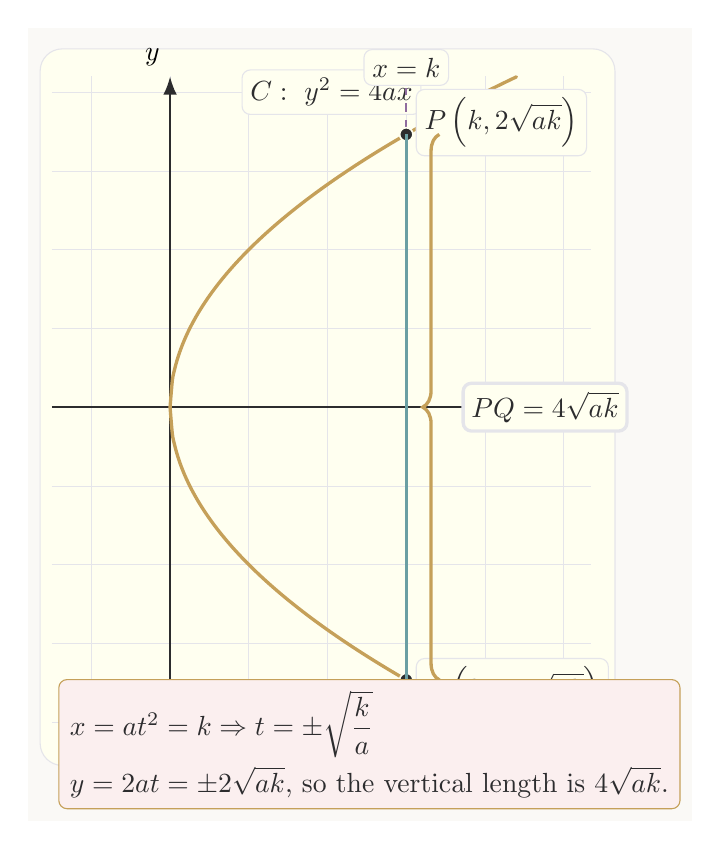
\begin{tikzpicture}[x=1cm,y=1cm,>=Latex,background rectangle/.style={fill=canvas},show background rectangle,
axis/.style={->,thick,draw=ink},gridline/.style={draw=linegray,line width=0.25pt},curve/.style={draw=gold,very thick,line cap=round},chord/.style={draw=teal,very thick},construction/.style={draw=purple,thick,dashed},point/.style={circle,fill=ink,draw=ivory,line width=0.6pt,inner sep=1.7pt},labelbox/.style={fill=ivory,draw=linegray,rounded corners=3pt,inner sep=3pt,align=left,text=ink},resultbox/.style={fill=rose,draw=gold,rounded corners=3pt,inner sep=4pt,align=left,text=ink}]
\pgfmathsetmacro{\kval}{3}
\pgfmathsetmacro{\yval}{2*sqrt(\kval)}
\fill[ivory,rounded corners=8pt,draw=linegray] (-1.65,-4.55) rectangle (5.65,4.55);
\foreach \x in {-1,0,...,5}{\draw[gridline] (\x,-4.2)--(\x,4.2);}
\foreach \y in {-4,-3,...,4}{\draw[gridline] (-1.5,\y)--(5.35,\y);}
\draw[axis] (-1.5,0)--(5.35,0) node[below right] {$x$};
\draw[axis] (0,-4.2)--(0,4.2) node[above left] {$y$};
\draw[curve,domain=0:4.4,samples=150,smooth,variable=\x] plot ({\x},{2*sqrt(\x)});
\draw[curve,domain=0:4.4,samples=150,smooth,variable=\x] plot ({\x},{-2*sqrt(\x)});
\node[labelbox] at (2.05,4.0) {$C:\ y^2=4ax$};
\draw[construction] (\kval,-4.05)--(\kval,4.05);
\node[labelbox,anchor=south] at (\kval,4.08) {$x=k$};
\coordinate (P) at (\kval,\yval); \coordinate (Q) at (\kval,-\yval);
\node[point] at (P) {}; \node[point] at (Q) {};
\node[labelbox,anchor=west] at ($(P)+(0.12,0.15)$) {$P\left(k,2\sqrt{ak}\right)$};
\node[labelbox,anchor=west] at ($(Q)+(0.12,-0.15)$) {$Q\left(k,-2\sqrt{ak}\right)$};
\draw[chord] (P)--(Q);
\draw[decorate,decoration={brace,amplitude=6pt},draw=gold,very thick] ($(Q)+(0.42,0)$)--($(P)+(0.42,0)$) node[midway,right=8pt,labelbox] {$PQ=4\sqrt{ak}$};
\node[resultbox,anchor=west] at (-1.42,-4.28) {$x=at^2=k\Rightarrow t=\pm\sqrt{\dfrac{k}{a}}$\\[2pt] $y=2at=\pm2\sqrt{ak}$, so the vertical length is $4\sqrt{ak}$.};
\end{tikzpicture}
\end{document}
